\documentclass[12pt]{article}
\usepackage[utf8]{inputenc}
\usepackage{float}
\usepackage{amsmath}
\usepackage{tikz}
\usepackage{graphicx}


\usepackage[hmargin=3cm,vmargin=6.0cm]{geometry}
\topmargin=-2cm
\addtolength{\textheight}{6.5cm}
\addtolength{\textwidth}{2.0cm}
\setlength{\oddsidemargin}{0.0cm}
\setlength{\evensidemargin}{0.0cm}
\usepackage{indentfirst}
\usepackage{amsfonts}

\begin{document}

\section*{Student Information}

Name : Gürhan İlhan Adıgüzel\\

ID : 2448025


\section*{Answer 1}
\paragraph{a)
\\\\Two continuous random variables are independent if the joint pdf is a product of marginal pdfs.
\\\\ Joint PDF : $\dfrac{1}{\pi}$
\\\\Hence the product of marginal PDFs is :\\
${\hspace*{50}}$ $f_X(x) f_y(y) = \dfrac{4}{\pi^2} \sqrt{(1-x^2)(1-y^2)} , {\hspace*{15}} -1 \leq x,y \leq 1$
\\\\Clearly, this is not equal to the joint PDF, and therefore, the two random variables are dependent.
}
\paragraph{b)
\\\\The Marginal PDF of X be found :
\\\\${\hspace*{50}}$ $f_{X}(x)$ = \(\int_{-\infty}^{\infty} f_{X,Y}(x,y) \,dy \) = \(\int_{-\sqrt{1-x^2}}^{\sqrt{1-x^2}} \dfrac{1}{\pi} \,dy\) = \dfrac{2}{\pi}\sqrt{1-x^2}, $\hspace*{25} -1 \leq x \leq 1 $
\\\\The Marginal PDF of Y be found : 
\\\\{\hspace*{50}} $f_{Y}(y)$ = \(\int_{-\infty}^{\infty} f_{X,Y}(x,y) \,dx \) = \(\int_{-\sqrt{1-y^2}}^{\sqrt{1-y^2}} \dfrac{1}{\pi} \,dx\) = \dfrac{2}{\pi}\sqrt{1-y^2}, \hspace*{25} -1 \leq y \leq 1
}
\paragraph{c)
\\\\{\hspace*{50}}${\mu}$ = E(X) = \(\int_{-1}^{1} x f_{X}(x) \,dx \) = \(\int_{-1}^{1} x \dfrac{2}{\pi}\sqrt{1-x^2} dx \) = 0
}
\paragraph{d)
\\\\ {\hspace*{50}}${\sigma^2}$ = Var(X) = \(\int_{-1}^{1} x^2f(x) dx\) - \mu^2 = \(\int_{-1}^{1} x^2 \dfrac{2}{\pi}\sqrt{1-x^2} dx \) = \dfrac{1}{4} - 0 = \dfrac{1}{4}
}
\newpage
\section*{Answer 2}
\paragraph{a)
\\\\ Joint Density Function:
\\\\ {\hspace*{50}}$f_{T_{a}} = 1/100 \hspace*{25} 0 \leq t_{a} \leq 100$  
\\\\ {\hspace*{50}}$f_{T_{b}} = 1/100 \hspace*{25} 0 \leq t_{b} \leq 100$
\\\\ {\hspace*{50}}$f_{T_{a}, T_{b}}(t_{a},t_{b})=\dfrac{d^2}{dt_{a}dt_{b}} F_{t_{a}, t_{b}}(t_{a},t_{b})= f_{T_{a}}(t_{a}) . f_{T_{b}}(t_{b})$
\\\\ {\hspace*{50}}$f_{T_{a}, T_{b}}(t_{a},t_{b}) = \dfrac{1}{100} . \dfrac{1}{100} =\dfrac{1}{10000} $
\\\\
\begin{equation*}
f(t_{a},t_{b}) = \left\{
\begin{array}{ll}
    \dfrac{1}{100} . \dfrac{1}{100} & \quad 0\leq t_{a} \leq 100 \hspace*{15} 0\leq t_{b} \leq 100\\\\
        0 & \quad otherwise\\
    \end{array}
\right.
\end{equation*}
\\\\Joint CDF :
\\\\Since $T_a$ and $T_b$ independent :
\\\\{\hspace*{50}}$F_{T_{a}, T_{b}}(t_{a}, t_{b}) =  P\{T_{a} \leq t_{a} \cap T_{b} \leq t_{b}\} $
\\\\{\hspace*{50}}$F_{T_{a}, T_{b}}(t_{a}, t_{b}) = F_{T_{a}} (t_{a}) . F_{T_{b}}(t_{b}).$
\\\\{\hspace*{50}}$F_{T_{a}} (t_{a}) = $\(\int_{0}^{100}  f(t_{a}) \,dt_{a}\) \hspace*{25} 
\\\\{\hspace*{50}}$F_{T_{b}}(t_{b}) =  $\(\int_{0}^{100}  f(t_{b}) \,dt_{b}\) \hspace*{25} 
\\\\{\hspace*{50}}$F_{T_{a}, T_{b}}(t_{a}, t_{b}) = $\(\int_{0}^{t_{a}} \int_{0}^{t_{b}} \dfrac{1}{100} . \dfrac{1}{100} \,dt_{a} dt_{b}\) $\hspace*{25} 0 \leq t_{a} \leq 100  \hspace*{25} 0 \leq t_{b} \leq 100$
\\\\{\hspace*{50}}$F_{T_{a}, T_{b}}(t_{a}, t_{b}) = \dfrac{t_{a} . t_{b}}{10000}$
\\\\\\\\ We can verify this formula with  : 
\\\\ {\hspace*{50}}F_{T_{a}, T_{b}}(t_{a}, t_{b}) = \(\int_{0}^{100} \int_{0}^{100} \dfrac{1}{100} . \dfrac{1}{100} \,dt_{a} dt_{b}\) = 1
}
\newpage
\paragraph{b)
\\\\We need to find A pushes the button in the first 10 seconds and subject B in the last 10 seconds with :
\\\\{\hspace*{50}} $P \{$T_{a}$ \leq 10\} =  F_{T_{a}} (10) = \int_{0}^{10} \dfrac{1}{100} \,dt_{a} = \dfrac{10}{100} $
\\\\{\hspace*{50}}$P\{$T_{b}$ \geq 90\} =  1- F_{T_{b}} (90) =\int_{0}^{90} \dfrac{1}{100} \,dt_{b} = 1 - \dfrac{90}{100} = \dfrac{10}{100}$
\\\\ Since $P(T_{a} \leq 10)$ and $P(T_{b} \geq 90) $ are independent :
\\\\ P\{$T_{a}$ \leq 10\} . P\{$T_{b}$ \geq 90\}  = F_{T_{a}} (10) . F_{T_{b}} (90)= \dfrac{10}{100} . \dfrac{10}{100} = \dfrac{1}{100}
}
\paragraph{c)
\\ {\hspace*{100}}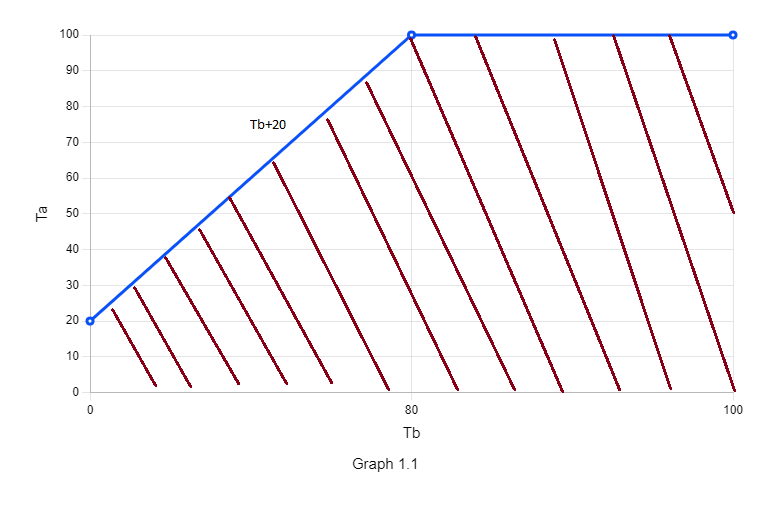
\includegraphics[scale=0.5]{Graph 1.1}
\\ According to the Graph 1.1 , we can divide this question into 2 parts :
\\\\ 1) In the first part we should consider that A pushes at most 20 seconds after B  for $T_{b}$ between 0 and 80 seconds. $T_{a}$ can take all the values between $[0 , t_{b}+20]$ So, 
\\\\ {\hspace*{50}} \(\int_{0}^{80} \dfrac{t_{b} + 20}{10000} dt_{b}\) = 0.48  {\hspace*{30}} $0\leq T_{b} \leq 80$
\\\\ 2) In the second part we should consider that when $T_{b}$ greater than 80 seconds, $T_{a}$ can take values between$[0,100]$ . So,
\\\\ {\hspace*{50}} \(\int_{80}^{100} \dfrac{100}{10000} dt_{b}\) = 0.20 {\hspace*{30}} $80\leq T_{b} \leq 100$
\\\\ As a result, when we sum this independent probabilities we can get : 
\\ {\hspace*{50}} P(1) + P(2) = 0.48 + 0.20 = 0.68
}
\newpage
\paragraph{d) 
\\\\ {\hspace*{100}}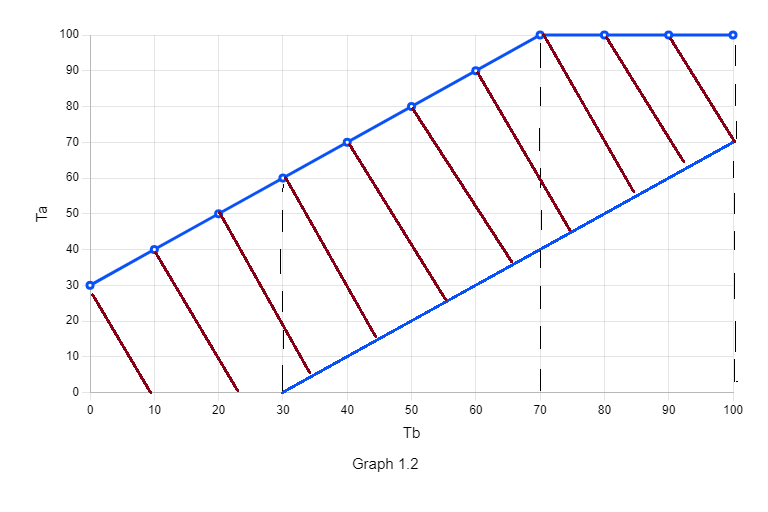
\includegraphics[scale=0.5]{Graph 1.2}
\\\\ According to the Graph 1.2,  we can divide this question into 3 parts :
\\\\ 1) In the first part we should consider that A can pushes a maximum of 30 seconds before or after from B. So, $T_{a}$ can take all the values between $[0,T_{b}+30]$ 
\\\\ {\hspace*{50}} \(\int_{0}^{30} \dfrac{t_{b} + 30}{10000} dt_{b}\) = 0.135  {\hspace*{30}} when {\hspace*{10}} 
$0\leq T_{b} \leq 30$
\\\\ 2) In the second part we should consider that when $T_{b}$ is between $(30,70)$, $T_{a}$ can take all the values between $[T_{b}-30, T_{b}+30]$. So,
\\\\ {\hspace*{50}} \(\int_{30}^{70} \dfrac{(t_{b} + 30) - (t_{b} - 30)}{10000} dt_{b}\) = \(\int_{30}^{70} \dfrac{60}{10000} dt_{b}\)= 0.240  {\hspace*{30}} when {\hspace*{10}}$30\leq T_{b} \leq 70$
\\\\ 3) In the third part we should consider that when $T_{b}$ is greater than 70, $T_{a}$ can take all tha values between $[T_{b}-30, 100]$. So,
\\\\ {\hspace*{50}} \(\int_{70}^{100} \dfrac{100 - (t_{b} - 30)}{10000} dt_{b}\) = \(\int_{70}^{100} \dfrac{130 - t_{b}}{10000} dt_{b}\) = 0.135  {\hspace*{30}} when {\hspace*{10}} $70\leq T_{b} \leq 100$
\\\\ As a result, when we sum this independent probabilities we can get : 
\\\\ {\hspace*{50}} P(1) + P(2) = 0.135+ 0.240 + 0.135 = 0.51
}
\newpage
\section*{Answer 3}
\paragraph{a)
\\\\ $F_{X_{i}}(x) = P(X_{i} \leq x) = 1- e^{-\lambda_{i} x_{i}}$
\\\\ Let T = min $\{X_{1}, X_{2}, . . . , X_{n}\}$. Then the cumulative distribution function of T
is:
\\\\ $F_{T}(y) = P(T \leq t)$
\\\\ {\hspace*{32}} = 1 - P(T \geq t)
\\\\ {\hspace*{32}} = 1 - P( min \{X_{1}, X_{2}, ..., X_{n}\} \geq t)
\\\\ {\hspace*{32}} = 1 - P(X_{1} \geq t, X_{2} \geq t, ..., X_{n} \geq t)
\\\\ {\hspace*{32}} = 1 - P(X_{1} \geq t) P(X_{2} \geq t)... P(X_{n} \geq t)
\\\\ {\hspace*{32}} = 1 - e^{-\lambda_{1}t} e^{-\lambda_{2}t}... e^{-\lambda_{n}t}
\\\\ {\hspace*{32}} = 1 - e^{-\lambda_{1}t -\lambda_{2}t...-\lambda_{n}t}
\\\\ {\hspace*{32}} = 1 - e^\[ -\sum_{i=1}^{n} \lambda_{i} t\] {\hspace*{50}} t $>$ 0
}
\paragraph{b)
\\\\ Let T = min $\{C_{1}, C_{2}, . . . , C_{10}\}$
\\\\ $F_{T}(t) = P(T \leq t)$
\\\\ {\hspace*{32}} = 1 - P(T \geq t)
\\\\ {\hspace*{32}}  = 1 - e^\[ -\sum_{n=1}^{10} \lambda_{n} y\] {\hspace*{50}} t $>$ 0
\\\\ e^\[ -\sum_{n=1}^{10} \lambda_{n} t\] = e^\[-(10/1) . t \]  . e^\[-(10/2) . t \]  ... e^\[-(10/10) . t \] 
\\\\ {\hspace*{32}}  =  1 -  e^\[-29.29 t \] 
}

\section*{Answer 4}
\subsection*{a)
\\\\ The number X of participants are undergraduate students has Binomial distribution with
\\\\ n = 100, p = 0.74, $\mu = np$ = 74, and $ \sigma =\sqrt{np . (1- p)} $= 4.386
\\\\ Applying the Central Limit Theorem with the continuity correction: 
\\\\ {\hspace*{50}}$P\{X \geq 70\} = P\{X > 69.5\} $= 1 - $P\{X < 69.5\}$
\\\\ {\hspace*{50}} $P\{X < 69.5\}$ = $P \{ \dfrac{X - 74}{\sqrt{74 . 0.26}}\} < P \{\dfrac{69.5-74}{\sqrt{74 . 0.26}}\} = \Phi(-1.02591)$ 
\\\\{\hspace*{50}} $P\{X > 69.5\} $ = $1 - \Phi(-1.02591)$
\\\\ {\hspace*{50}}$\Phi(-1.02591) = 0.1525 $
\\\\ {\hspace*{50}} $P\{X < 69.5\}$ == $1- 0.1525 = 0.8485 $
}
\subsection*{b)
\\\\ The number X of participants are pursuing a doctoral degree has Binomial distribution with
\\\\ n = 100, p = 0.10, $\mu = np$ = 10, and $ \sigma =\sqrt{np . (1 - p)} $= 3
\\\\Applying the Central Limit Theorem with the continuity correction: 
\\\\{\hspace*{50}}$P\{X \leq 5 \} = P\{X < 5.5\} $ = $P \{ \dfrac{X - 10}{\sqrt{10 . 0.9}}\} < P \{\dfrac{5.5-10}{\sqrt{10 . 0.9}}\}$ = $\Phi(-1.5)$
\\\\ {\hspace*{50}}$\Phi(-1.5) = 0.066807 $
}
\end{document}

